% Copyright (C) 2022 Haoqing Xu
% School of Artificial Intelligence, Southeast University.
% --------------------------------------------------------------------------
%
% This work may be distributed and/or modified under the
% conditions of the LaTeX Project Public License, either
% version 1.3c of this license or (at your option) any later
% version. This version of this license is in
%    http://www.latex-project.org/lppl/lppl-1-3c.txt
% and the latest version of this license is in
%    http://www.latex-project.org/lppl.txt
% and version 1.3 or later is part of all distributions of
% LaTeX version 2005/12/01 or later.
%
% This work has the LPPL maintenance status `maintained'.
% The Current Maintainer of this work is Haoqing Xu.
%
% Home Page of the Project: https://github.com/SuikaXhq/seu-bachelor-thesis-2022
\documentclass{seuthesis-2022}

\title{}{（此栏可删除）}
\author{}
\studentnum{}
\department{}
\major{}
\supervisor{}
\period{}

\begin{document}

\maketitle
\makedeclaration

\frontmatter
\begin{abstract}[zh]
  摘要内容独立于正文而存在，是论文内容高度概括的简要陈述，应准确、具体、完整地概括论文的主要信息，内容包括研究目的、方法、过程、成果、结论及主要创新之处等，不含图表，不加注释，具有独立性和完整性，一般为400字左右。
  
  “摘要”用三号黑体加粗居中，“摘”与“要”之间空4个半角空格。摘要正文内容用小四号宋体，固定1.5倍行距。
  
  论文的关键词是反映毕业设计（论文）主题内容的名词，一般为3-5个，排在摘要正文部分下方。关键词与摘要之间空一行。关键词之间用逗号分开，最后一个关键词后不加标点符号。
  \keywords{关键词1,关键词2,关键词3,关键词4}
\end{abstract}

\begin{abstract}[en]
  英文摘要应与中文摘相对应，250个实词左右。采用第三人称介绍该学位论文内容，叙述的基本时态为一般现在时，确实需要强调过去的事情或者已经完成的行为才使用过去时、完成时等其他时态。
  
  ABSTRACT为三号Times New Roman加粗居中。
  
  英文摘要正文为小四号Times New Roman，固定1.5倍行距。英文关键词“KEY WORDS”大写，其后的关键词第一个字母大写，关键词之间用半角逗号隔开。
  \keywords{Keywords1,Keywords2,Keywords3,Keywords4}
\end{abstract}

\tableofcontents

\mainmatter
\chapter{绪论}
\section{课题背景和意义}
\subsection{课题背景} 
近年来，随着实时交互和多媒体应用的快速发展，如远程协作平台、智能监控系统、云存储[1] 等，网络传输需求呈现出爆发式增长。这些应用对数据传输的带宽、延迟和可靠性提出了更高的要求[2] [3]。与此同时，5G、WiFi 6、WiFi 7以及未来的6G[4] 等新一代通信技术的迅速普及，显著提升了无线空口的传输速率，理论上可以达到10Gbps以上。然而，随着无线带宽大幅增加，传统的TCP/IP协议栈的弊端逐渐凸显。实时4K视频需要至少每秒30帧，这意味着对于每一帧，包括编码，传输和解码的处理过程必须在60 ms内完成，即使不考虑传输延迟，4K视频的基于软件协议栈的编解码器延迟（180-250 ms）也远超可容忍的范围。其对终端CPU的大量占用和消耗，无法和链路的高速率保持同步，同时CPU容易由于高负载加热降频，由于木桶效应，整个网络的带宽取决于链路上各点的最小值，因此端侧性能制约了整个网络的性能。

在这一背景下，RDMA（remote direct memory access, 远程直接内存访问）技术[5] 为解决上述问题提供了新的思路。RDMA的核心原理是通过绕过操作系统内核，直接在应用程序的内存之间传输数据，从而减少CPU的干预和数据处理开销。传统的数据传输方式需要CPU参与数据的复制、校验和协议处理等操作，这不仅增加了CPU的负载，还引入了额外的延迟。而RDMA利用Kernel Bypass（内核旁路）和Zero Copy（零拷贝）技术，实现了低延迟、高吞吐量的数据传输，同时显著降低了CPU的负载。

RDMA技术将数据传输任务卸载到网卡，CPU仅需负责控制面的交互，使得数据可以直接从发送端的内存传输到接收端的内存，这种方式不仅减少了CPU的负担，还大大降低了数据传输的延迟。对于高带宽、低延迟的应用场景，如大规模数据中心、高性能计算、实时视频流处理等，RDMA技术能够显著提升传输效率，极大优化了协议栈处理速度。
在数据中心的有线网络场景下，RDMA已经被实践证明出其有效性[6] [7]，实现了大规模的部署。在无线场景中，随着无线带宽的不断提升，RDMA技术为解决无线场景下终端CPU性能瓶颈提供了一种可能的高效解决方案。

\subsection{课题意义} 
RDMA目前仅大规模应用于数据中心的有线场景中，本课题为RDMA未来在无线领域的应用给出了新的见解和思路。虽然本课题的无线协议栈仅使用了5G，但是具有广阔的探索空间：
\begin{itemize}
    \item 5G协议作为目前（截止至2025.4）带宽最大、时延最低[] 的无线协议，是在应用场景中最迫切需要端侧处理时延下降来达到与链路速率匹配的协议，因此我们使用5G协议栈开展研究；
    \item 鉴于本课题提出的算法并没有利用5G协议相较之其他802.11协议的特殊特性，因此本算法并不局限于在5G协议栈上使用，但由于其他协议（如WLAN）超出本课题的研究范围，遂没有给出实验验证；
    \item 对于未来可能出现的、更高速的无线协议（如6G[] ），本课题为这些无线协议与RDMA等端侧加速技术的结合使用给出了一些速率控制的算法思路；
    \item 本课题提出的速率控制算法考虑到无线段速率与有线段不匹配的问题，针对原生RDMA速率控制算法给出了改进和优化，缩短了速率控制路径，对于未来异构链路的速率控制算法的设计给出了新的解决思路。
\end{itemize}

\section{研究现状}
本文创新性的将RDMA技术应用到无线场景当中，作为面向未来高速无线链路的预言性质研究，我们聚焦于5G协议栈和RDMA协议栈的结合。随着网络应用对时延和带宽的要求逐渐提升，学术界和产业界对RDMA和5G技术都有较为深入的研究，下面分别对这两种技术迄今的研究现状进行分析和总结，最后也给出无线RDMA的相关研究。

\subsection{RDMA技术}
\subsubsection{RDMA技术兴起的背景与应用价值}
随着云计算、人工智能模型训练等应用的快速发展，数据中心网络需要承载的应用对网络延迟和带宽的要求日益提升，传统TCP/IP网络架构的传输效率逐渐成为瓶颈。例如在大模型的训练和推理任务中，训练任务的特点是大数据量，对网络的要求是大带宽，而传统的基于socket的网络结构需要数据从应用层拷贝到内核层，大数据量的拷贝严重拖慢了效率；推理任务的特点是小数据量，对网络的要求是低时延，传统的TCP/IP架构不仅需要经过软件协议栈的层层处理，每发送一次数据都要产生一个CPU中断，大大增加了时延。

因此，为了解决传统协议栈数据拷贝代价大、软件处理速度慢的问题，RDMA技术应运而生。RDMA通过​​零拷贝​和​​内核旁路​​机制，允许网卡绕过操作系统内核直接访问用户态内存，从而将数据传输延迟降，同时释放了大量的CPU资源。其在数据中心网络中已经实现了大规模应用，下文给出一些RDMA的实际应用场景。

\begin{itemize}
    \item ​​云原生计算​​：在容器化微服务架构中，RDMA支撑了Kubernetes集群的跨节点高效通信，例如微软Azure的HPC云服务部署了RoCEv2网络，实现了虚拟机间延迟敏感型任务的性能飞跃。
    \item ​​分布式存储系统​​：结合NVMe-oF（NVMe over Fabrics）协议，RDMA使得全闪存存储池的IOPS（每秒输入输出操作次数）提升至百万级别，Ceph、IBM Spectrum Scale等分布式存储系统通过RDMA优化可实现亚毫秒级块存储访问。
    \item ​​AI训练集群​​：RDMA技术承载了GPU间数据传输的任务，为此也提出了一些GPU数据传输专门化的技术标准，例如NVIDIA的GPUDirect RDMA技术允许RDMA直接从GPU显存中取数据，不需要经过主机内存中转，将大规模模型训练的通信开销降低50\%以上，在各种大模型训练和推理显著提升了效率。
    \item ​​金融高频交易​​：证券交易系统通过RDMA实现纳秒级行情分发，伦敦证券交易所的“Millennium Exchange”平台采用Mellanox RDMA技术将订单处理延迟压缩至800纳秒。
\end{itemize}

\subsubsection{RDMA核心技术原理}
RDMA的操作分为RDMA READ、RDMA WRITE、RDMA SEND等，
\begin{figure}[h] % 'h' 表示图形尽量在当前位置显示
    \centering % 图形居中
    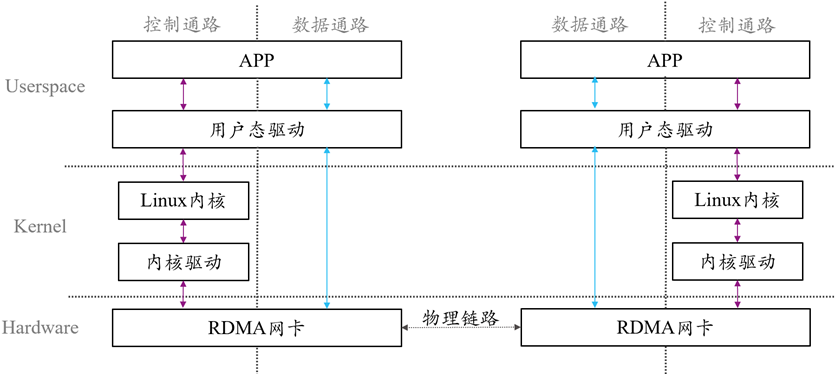
\includegraphics[width=0.80\textwidth]{fig/RDMA原理.png} % 插入图片，调整宽度为文本宽度的80%
    \caption{RDMA技术原理}
    \label{figRDMA_tech}
\end{figure}
如图\ref{figRDMA_tech}，RDMA实现了以下几个特点：
\begin{itemize}
    \item CPU Offload：指的是RDMA的数据读写过程无需CPU干预。在RDMA初始化的时候，进行通信的RDMA端点将会注册一块RDMA对端可以访问的数据内存（MR,memory region）信息，并将其页表存储在网卡硬件中，同时会pin住这块内存，禁止这块内存被置换出去。后续数据的读写操作完全不需要CPU介入，借助底层的DDP（direct data placement）技术，直接对这块内存进行数据的读写。这样不仅可以减少CPU资源消耗，降低时延，同时远程主机的CPU的缓存不会被访问的内存内容所污染。
    \item Kernel Bypass：RDMA 为用户提供了一套专有的 Verbs interface 而不是传统的TCP/IP Socket interface，减少了用户态和内核态上下文切换的延迟。
    \item Zero Copy：需要进行网络传输的应用数据不需要先从应用层被搬运到内核层，而是可以直接在用户态执行数据传输，减少了数据搬运的时间，
\end{itemize}
\subsubsection{RDMA技术分类}
iWARP、RoCE和InfiniBand是三种主流的RDMA实现技术。iWARP基于TCP/IP协议栈，通过TOE技术实现CPU卸载，支持跨广域网传输但延迟较高；RoCE则基于以太网，分为RoCEv1和RoCEv2两个版本，其中RoCEv1仅支持二层网络，而RoCEv2通过UDP/IP实现三层路由并引入ECN/PFC等拥塞控制机制；InfiniBand作为专用网络协议，采用独立的网络架构，提供极低延迟和高吞吐，但需要从网卡到交换机全套的专用硬件支持，价格昂贵。目前大型数据中心中使用最广泛的是RoCEv2协议，这也是本文选择的仿真实现技术。

\subsubsection{RDMA现有的拥塞控制和流量管理机制}
RDMA与TCP不同，因其原生的丢包恢复机制是GBN(go-back-N)，一旦丢包，恢复代价极大，因此它需要一个\textbf{无损网络}。​​无损传输​​与​​低延迟​​的核心目标对拥塞控制、流量调度和丢包的恢复机制提出了严苛的要求。传统TCP的端到端拥塞控制策略难以适应RDMA的微秒级延迟需求，因此业界提出了多种创新设计，本节将重点解析IRN、DCQCN等机制的核心原理与应用场景。

\textbf{IRN}
来自sigcomm'18的文章提出了一个名为Improved RoCE NIC（IRN）的设计，IRN对于现在的RDMA网卡改进主要是以下几点：
\begin{itemize}
    \item 改进了丢包恢复机制（从原生的Go-back-N算法改进为Selective-repeat算法）。接收方不会像Go-back-N中一样丢弃乱序的数据包，而是将其暂存。而发送方在确认数据包丢失后会选择性地重传那些丢失的数据包，这要求发送方维护一个位图，记录已发送数据包的状态。
    \item 添加了基本的端到端流量控制，称为BDP-FC，通过网络中的带宽时延积（BDP）来限制网络的流中在途的未处理的数据包的数量。
\end{itemize}
\textbf{DCQCN}
DCQCN是目前各个数据中心网络应用最广泛、效果最好的拥塞控制算法，其设计主要包含以下几个部分：
\begin{itemize}
    \item ECN标记与量化反馈​​：交换机在检测到队列拥塞时，对数据包头部的ECN位打标，当接收端接收到携带ECN标记的数据包后，发送CNP（Congestion Notification Packet）来向发送端反馈拥塞程度（量化值Q），发送端随之降速。
    \item 多级速率调整​​：发送端根据CNP的量化Q值动态调整速率，分为快速恢复（Fast Recovery）、主动减速（Active Backoff）和稳定态（Additive Increase）三个阶段，来达到保持网络中数据量的相对稳定。
\end{itemize}
本文的算法设计基于DCQCN，针对无线场景做出了定制化修改。
\subsection{5G技术}
\subsubsection{5G技术概览}
5G技术在本文撰写时，仍是现有通信协议栈中最高速的协议，最新协议中要求5G的上行速率达到10Gbps，下行速率达到20Gbps。当前，5G技术已进入规模化商用阶段，全球主要国家已经基本完成了核心城市覆盖，中国更部署了超300万个基站。其核心技术包含毫米波、Massive MIMO和网络切片，实现了增强移动宽带（eMBB）、超高可靠低时延（uRLLC）与海量机器通信（mMTC）三大场景。5G与工业互联网、车联网（C-V2X）、AR/VR实现了深度融合，推动智能制造、远程医疗等行业的数字化转型。
\subsubsection{5G协议栈的重传机制——HARQ}
5G使用的重传恢复机制为HARQ（混合自动重传请求，Hybrid Automatic Repeat reQuest），由ARQ（自动重传请求，Automatic Repeat-reQuest）和FEC（前向纠错码，Forward Error Correction）两种方案结合组成。

ARQ机制通过接收端的错误检测反馈触发数据重传，确保可靠性，但对网络时延敏感；​FEC在发送端添加冗余纠错码，接收端直接纠错，不需要重传，适合用于高时延或实时场景（如语音传输）。

HARQ系统则结合二者的优势，由一个包含在ARQ系统中的FEC子系统组成。该方法通过对频繁出现的错误进行修正，从而减少了平均重传次数。当检测到较低频率的错误时，接收方会请求重传，其中每次重传都携带一些冗余信息，以帮助数据包恢复。HARQ使用FEC来纠正接收端部分错误，并依靠错误检测来检测剩余的错误。在增量冗余HARQ方案中（HARQ-IR），每次重传后，接收端都能获得更丰富的奇偶校验位集，提高了可靠解码的概率。
\subsubsection{RLC层的两种传输模式：UM\&AM}
\begin{figure}[h] % 'h' 表示图形尽量在当前位置显示
    \centering % 图形居中
    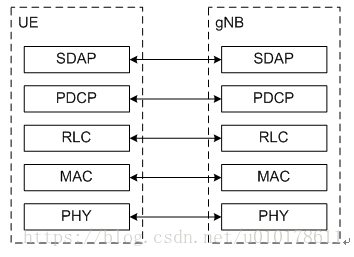
\includegraphics[width=0.80\textwidth]{fig/5G协议栈.png} % 插入图片，调整宽度为文本宽度的80%
    \caption{5G协议栈}
    \label{5Glayer}
\end{figure}
如图\ref{5Glayer}，展示了5G的协议栈结构，SDAP层上面就是用户数据（IP数据或非IP数据）。这里单独介绍一下RLC层。无线链路控制协议（RLC）是为了保证数据传输业务可靠服务质量（QoS）而制定的协议。RLC层位于MAC层（Medium Access Control，媒体访问控制层）的上方，MAC层通过控制底层的物理层媒介传递数据，把逻辑信道数据映射到传输信道，并把映射后的传输信道的传输块数据（TB，transmission block）传递给物理层，因此RLC层和MAC之间交换的数据是以传输块的形式出现。

RLC一般有几种传输模式，有损无线协议（UM模式，unacknowledged mode）和无损无线协议栈（AM模式，acknowledged mode）。

非确认模式UM（UnacknowIedged Mode）—— 类UDP模式（RLC不做重传ARQ处理）
\begin{itemize}
\item UM数据传输能够保证数据按序传递给上层，并且能够对上层数据根据无线资源的带宽限制进行打包分段，以最短时延使数据包按序到达对端，主要适用于对时延敏感、但是允许一定丢包率的业务。
\item 在发送端，UM发送实体通过其与上层协议栈之间的服务接入点SAP（service access point, 类似TCP/IP socket）将上层数据放入发送缓存队列中，然后根据MAC层给予的发送机会（发送机会信息中携带允许发送给的最大字节数）对发送缓存中的数据进行打包分段，最后加上 RLC头，通过逻辑信道发送出去。
\end{itemize}
确认模式AM（Acknowledged Mode）—— 类TCP模式（RLC提供重传）
\begin{itemize}
    \item AM数据传输以ARQ的方式为上层提供可靠的数据传输，保证数据正确地按序到达对端，主要适用于时延不敏感、对错误敏感的业务，如FTP业务、后台业务、交互业务等。
    \item 在AM模式中，由发送端和接收端共同完成 ARQ差错控制过程，完成重排序、重组等功能，这是RLC层一个重要的功能。
\end{itemize}
\subsection{无线RDMA}
关于RDMA在有线领域的研究已经有了很多成果，但是对于RDMA在无线领域的应用较少，没有非常成熟的研究。通过调研，工作[9]首次提出了无线-RDMA（W-RDMA）的概念。
\begin{figure}[h] % 'h' 表示图形尽量在当前位置显示
    \centering % 图形居中
    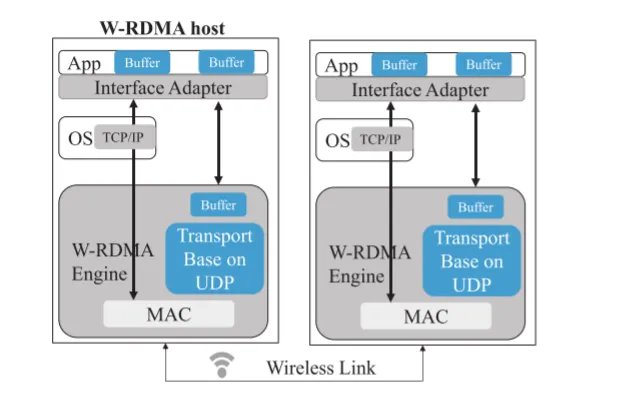
\includegraphics[width=0.80\textwidth]{fig/WRDMA.png} % 插入图片，调整宽度为文本宽度的80%
    \caption{W-RDMA}
    \label{WRDMA}
\end{figure}
这篇论文首次提出了RDMA在无线领域的应用可能性，如图\ref{WRDMA}，设计了一个W-RDMA引擎，这个引擎在硬件空间中实现，包含一个主机信道适配器以自动选择合适的无线信道、一个速率控制器和丢包恢复模块，下层使用UDP协议作为载体传输。

该工作简单描述了W-RDMA的框架，在WLAN上做了简单的探索，并没有明确给出W-RDMA引擎的设计细节，从吞吐量上看也没有达到非常优异的效果，但是为未来RDMA应用于无线领域提供了新的思路。

\section{本文研究内容}
目前，还没有对于RDMA应用于无线领域的成熟研究，本文的研究目标是使用ns-3网络仿真工具，基于目前速率最快的无线协议5G标准，将端侧的TCP/IP协议栈替换成RDMA协议栈，并实现出一种适用于无线有线相结合场景下的速率控制算法。在前述研究的基础上，本课题面临的\textbf{挑战}主要来自于以下几个方面：
\begin{itemize}
    \item \textbf{使用ns-3搭建RDMA和5G协议栈结合的网络拓扑的复杂性：}使用ns-3仿真实现的RDMA协议栈和5G协议栈已有可参考的项目，但是如何将两种完全不同性质的协议栈融合实现仿真是具有挑战性的；
    \item \textbf{无线段和有线段速率不匹配问题：}尽管选择了较为高速的5G标准，以太网的链路速率仍然远高于无线链路速率，这种速率差会在中间网络节点上产生较为严重的网络拥塞，如何设计合适的速率控制算法并实现之是一个需要解决的挑战；
    \item \textbf{}
\end{itemize}
\chapter{正文}
正文部分每一章应另起页书写书写，层次要清楚，内容要有逻辑性，正文一般不少于15000字。正文部分因学科、选题特点可有差异，但必须言之成理，论据可靠，严格遵循本学科国际通行的学术规范。

中文为小四号宋体，英文及数字为小四号Times New Roman，首行缩进2个字符，行间距为1.5倍。

\section{插图格式要求}
插图力求精炼，且每个插图均应有图序和图名。图序与图名位于插图下方，图序一般按章节编排，如图1-1（第一章第1个图），在插图较少时可以全文连续编序，如图10。

如一个插图由两个及以上的分图组成，分图用(a)、(b)、(c)等标出，并标出分图名。

简单文字图可用WORD直接绘制，复杂的图考虑使用相应的图形绘制软件完成，以提高图形表达质量。

插图居中排列，与上文文本之间空一行。图序图名设置为五号宋体居中，图序与图名之间空一格。

引用：图 \ref{fig:1}、图 \ref{fig:2}、图 \ref{fig:2a}、图 \ref{fig:2b} 的引用示例（见tex文件）。

\begin{figure}[H]
    \centering
    \includegraphics[width=0.5\linewidth]{fig/降水量均值分布图.png}
    \caption{每小时降水量24小时均值分布图}
    \label{fig:1}
\end{figure}

\begin{figure}[H]
    \centering
    \subcaptionbox{速度障碍集合\label{fig:2a}}
      {\includegraphics[width=0.3\linewidth]{fig/速度障碍集合.png}}
    \subcaptionbox{速度障碍集合\label{fig:2b}}
      {\includegraphics[width=0.4\linewidth]{fig/避免碰撞集合.png}}
    \caption{速度障碍法速度选择}
    \label{fig:2}
\end{figure}

\section{表格格式要求}
表格的结构应简洁，一律采用三线表，应有表序和表名，且表序和表名位于表格上方。表格可以逐章单独编序（如：表2.1），也可以统一编序（如：表10），采用哪种方式应和插图及公式的编序方式统一。表序必须连续，不得重复或跳跃。

表格无法在同一页排版时，可以用续表的形式另页书写，续表需在表格右上角表序前加“续”字，如“续表2.1”，并重复表头。

表格居中，边框为黑色直线1磅，中文为五号宋体，英文及数字为五号Times New Roman字体，表序与表名之间空一格，表格与下文之间空一行。需要注意必须在tabular环境前手动指定字号（见tex文件）。

引用：表 \ref{tab:1} 的引用示例（见tex文件）。

\begin{table}[H]
  \centering
  \caption{降水率分级统计}
  \label{tab:1}
  \small
  \begin{tabular}{ccc}
    \toprule
    降水率(mm/h)分级 & 该等级所占比例(\%) & 降水等级描述\\
    \midrule
    $0\le x< 0.5$ & 90.36 & 没有雨或雨很小\\
    $0.5\le x< 2.0$ & 6.41 & 小雨\\
    $2.0\le x< 5.0$ & 2.04 & 中雨\\
    $5.0\le x< 10.0$ & 0.10 & 大雨\\
    \bottomrule
  \end{tabular}
\end{table}

\section{表达式}
论文中的公式应注序号并加圆括号，序号一律用阿拉伯数字连续编序（如（28））或逐章编序（如（3.6）），编号方式应与插图、表格方式一致。序号排在版面右侧，且距右边距离相等。公式与序号之间不加虚线。

长公式在一行无法写完的情况下，原则上应在等号（或数学符号，如“+”、“-”号）处换行，数学符号在换行的行首。

公式及文字中的一般变量（或一般函数）（如坐标X、Y，电压V，频率f）宜用斜体，矢量用粗斜体如S或白斜体上加单箭头，常用函数（如三角函数cos、对数函数ln等）、数字运算符、化学元素符号及分子式、单位符号、产品代号、人名地名的外文字母等用正体。

公式排版时可选中模板中的“公式式样”，先将光标移至公式前，按“Tab”键，公式居中；再将光标移至编号前，按“Tab”键移动一个制表符位置，使公式编号右对齐。
\begin{equation}\label{eq:1}
  V_{cell}=E_{OCV}-V_{oct}-V_{ohm}-V_{conc}
  \end{equation}
引用：公式 \eqref{eq:1} 的引用示例（见tex文件）。

  
\section{注释}
正文中有个别名词或情况需要解释时，可加注说明，注释采用页末注（将注文放在加注页的下端）。在引文的右上角标注序号\circled{1}、\circled{2}、……，如“马尔可夫链\footnote{马尔科夫链表示}”。若在同一页中有两个以上的注时，按各注出现的先后，顺序编号。引文序号，以页为单位，且注释只限于写在注释符号出现的同页，不得隔页。

注释采用小五号宋体，英文及数字为小五号Times New Roman字体，利用“引用”插入脚注功能插入。

\chapter{总结与展望}
\section{工作总结}
最后一章结论与展望着重总结论文的创新点或新见解及研究展望或建议。

结论是对论文主要研究结果、论点的提炼与概括，应准确、简明、完整、有条理，使人看后就能全面了解论文的意义、目的和工作内容。主要阐述自己的创造性工作及所取得的研究成果在本学术领域中的地位、作用和意义。

结论要严格区分自己取得的成果与导师及他人的科研工作成果。在评价自己的研究工作成果时，要实事求是，除非有足够的证据表明自己的研究是“首次”的、“领先”的、“填补空白”的，否则应避免使用这些或类似词语。

\section{工作展望}
展望或建议，是在总结研究工作和现有结论的基础上，对该领域今后的发展方向及重要研究内容进行预测，同时对所获研究结果的应用前景和社会影响加以评价，从而对今后的研究有所启发。

\nocite{*}
\bibliographystyle{gbt7714-numerical}
\bibliography{reference.bib}

\appendix
\chapter{附录名称}
对于一些不宜放入正文中、但作为毕业设计（论文）又不可残缺的组成部分或具有重要参考价值的内容，可编入毕业设计（论文）的附录中，例如，正文内过于冗长的公式推导、方便他人阅读所需的辅助性数学工具或表格、重复性数据和图表、非常必要的程序说明和程序全文、关键调查问卷或方案等。

附录的格式与正文相同，如有多个附录需依顺序用大写字母A，B，C，……编序号，如附录A，附录B，附录C，……。只有一个附录时也要编序号，即附录A。每个附录应有标题，如：“附录A 参考文献著录规则及注意事项”。

附录一般与论文全文装订在一起，与正文一起编页码。


\begin{acknowledgement}
学位论文正文和附录之后，一般应放置致谢（后记或说明），主要是感谢指导老师和对论文工作有直接贡献和帮助的人士和单位。致谢言语应谦虚诚恳，实事求是。字数一般不超过1000个汉字。

“致谢”用三号黑体加粗居中，两字之间空4个半角空格。致谢内容为小四号宋体，1.5倍行距。
\end{acknowledgement}
\end{document}